\documentclass[11pt]{standalone}
\usepackage{amssymb}
\usepackage{amsmath}

\usepackage[no-math]{fontspec}
\usepackage{unicode-math}
\setmainfont{Libertinus Sans}
\setsansfont{Libertinus Sans}
\setmathfont{Libertinus Math}

\usepackage{pgf,xcolor}
\usepackage{tikz}
\usetikzlibrary{arrows.meta, backgrounds}
\usepackage{pgfplots}
\pgfplotsset{compat=newest}

\definecolor{my_darkgray}{HTML}{484949}
\definecolor{my_lightgray}{HTML}{F3F4F4}
\definecolor{my_darkblue}{HTML}{005A94}
\definecolor{my_lightblue}{HTML}{CCDEE9}
\definecolor{my_yellow}{HTML}{FFEC7F}
\definecolor{my_red}{HTML}{E60000}
\definecolor{my_orange}{HTML}{E87846}

\begin{document}
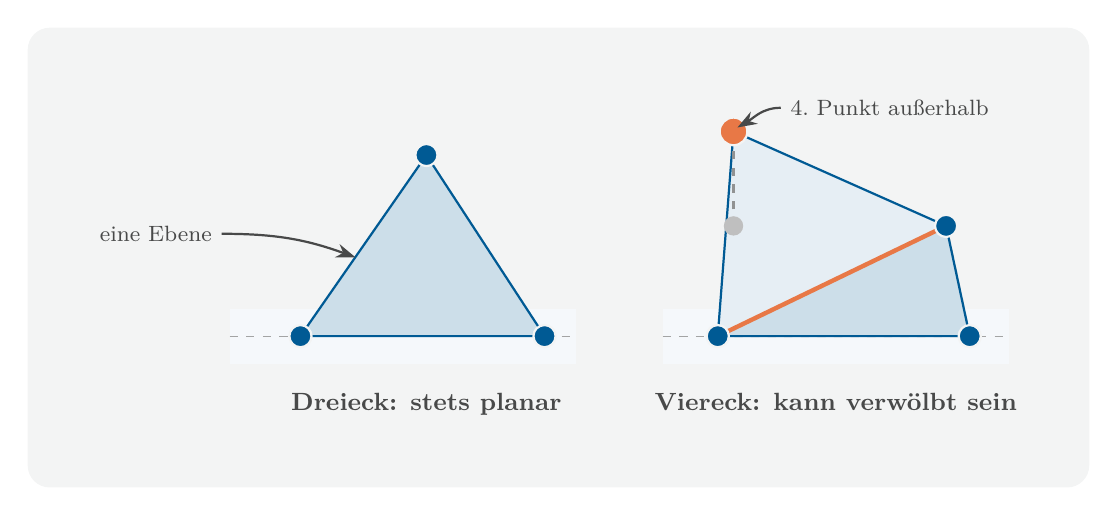
\begin{tikzpicture}[
    show background rectangle,
    background rectangle/.style={fill=my_lightgray, rounded corners=8pt},
    inner frame sep=0.8cm,
    annotation/.style={draw=my_darkgray, thick, -{Stealth[length=7pt, width=5pt]}}
]

% ================================================================
% LINKES PANEL: Dreieck (stets planar)
% ================================================================

% Referenzebene (dezenter horizontaler Streifen bei y=0.5)
\fill[my_lightblue!20] (-0.2, 0.15) rectangle (4.2, 0.85);
\draw[my_darkgray!50, dashed] (-0.2, 0.5) -- (4.2, 0.5);

% Dreieck-Vertices
\coordinate (A) at (0.7, 0.5);
\coordinate (B) at (3.8, 0.5);
\coordinate (C) at (2.3, 2.8);

% Füllung und Kontur
\fill[my_lightblue] (A) -- (B) -- (C) -- cycle;
\draw[my_darkblue, thick] (A) -- (B) -- (C) -- cycle;

% Vertices
\foreach \v in {A, B, C} {
    \fill[my_darkblue] (\v) circle (4pt);
    \draw[my_lightgray, thick] (\v) circle (4pt);
}

% Annotation: alle 3 Punkte in der Ebene
\node[font=\footnotesize, text=my_darkgray, anchor=east] (lbl_tri)
    at (-0.3, 1.8) {eine Ebene};
\draw[annotation] (lbl_tri.east) to[out=0, in=160] (1.4, 1.5);

% Panel-Titel
\node[font=\small\bfseries, text=my_darkgray, anchor=north] at (2.3, -0.1)
    {Dreieck: stets planar};

% ================================================================
% RECHTES PANEL: Viereck (kann verwölbt sein)
% ================================================================
\begin{scope}[xshift=5.5cm]

% Referenzebene
\fill[my_lightblue!20] (-0.2, 0.15) rectangle (4.2, 0.85);
\draw[my_darkgray!50, dashed] (-0.2, 0.5) -- (4.2, 0.5);

% Viereck-Vertices
\coordinate (P1) at (0.5, 0.5);   % unten links  (in der Ebene)
\coordinate (P2) at (3.7, 0.5);   % unten rechts (in der Ebene)
\coordinate (P3) at (3.4, 1.9);   % oben rechts  (in der Ebene)
\coordinate (Pflat) at (0.7, 1.9);% oben links   (in der Ebene, Geisterpunkt)
\coordinate (P4)    at (0.7, 3.1);% oben links   (verwölbt, tatsächliche Position)

% Gestrichelter Geist-Umriss (flaches Viereck, wie es wäre)
\draw[my_darkgray!40, dashed, thick] (P1) -- (P2) -- (P3) -- (Pflat) -- cycle;

% Tatsächliche untere Dreiecksfläche P1-P2-P3 (in der Ebene)
\fill[my_lightblue]     (P1) -- (P2) -- (P3) -- cycle;
\draw[my_darkblue, thick] (P1) -- (P2) -- (P3) -- cycle;

% Tatsächliche obere Dreiecksfläche P1-P3-P4 (verwölbt)
\fill[my_lightblue!50]  (P1) -- (P3) -- (P4) -- cycle;
\draw[my_darkblue, thick] (P1) -- (P3) -- (P4) -- cycle;

% Faltlinie P1-P3 (der Knick, my_orange)
\draw[my_orange, ultra thick] (P1) -- (P3);

% Höhenindikator: gestrichelter Pfeil von Geisterpunkt zu P4
\draw[my_darkgray!60, dashed, thick] (Pflat) -- (P4);
\fill[my_darkgray!35] (Pflat) circle (3.5pt);

% Vertices
\foreach \v in {P1, P2, P3} {
    \fill[my_darkblue] (\v) circle (4pt);
    \draw[my_lightgray, thick] (\v) circle (4pt);
}
% Verwölbter Vertex P4 (my_orange)
\fill[my_orange] (P4) circle (5pt);
\draw[my_lightgray, thick] (P4) circle (5pt);

% Annotation: verwölbter Vertex
\node[font=\footnotesize, text=my_darkgray, anchor=west] (lbl_p4)
    at (1.3, 3.4) {4.~Punkt außerhalb};
\draw[annotation] (lbl_p4.west) to[out=180, in=30] (0.75, 3.15);

% Panel-Titel
\node[font=\small\bfseries, text=my_darkgray, anchor=north] at (2.0, -0.1)
    {Viereck: kann verwölbt sein};

\end{scope}

\end{tikzpicture}
\end{document}
